\section{SLAM and Navigation}
\subsection{2D SLAM}
%=========================================================================================================================
%-------------- SLAM_TOOLBOX
%=========================================================================================================================
\subsubsection*{slam\_toolbox}
The slam\_toolbox package incorporates information from laser scanners in the form of a LaserScan message and TF transforms from \textcolor{Violet}{\texttt{odom->base\_link}}, and creates a map 2D map of a space. This package will allow you to fully serialize the data and pose-graph of the SLAM map to be reloaded to continue mapping, localize, merge, or otherwise manipulate. We allow for SLAM Toolbox to be run in synchronous (process all valid sensor measurements, regardless of lag) and asynchronous (process valid sensors measurements on an as-possible basis) modes.\\

slam\_toolbox provides various tools and capabilities to address the problems with SLAM, and it offers several features:

\begin{itemize}
    \item \textit{\textbf{Basic 2D SLAM for Mobile Robotics}}: slam\_toolbox allows users to perform standard point-and-shoot 2D SLAM, where a mobile robot explores the environment, builds a map, and saves it in PGM (Portable Graymap) file format. The library also includes utilities to facilitate map saving.
    
    \item \textit{\textbf{Continuing and Refining Mapping}}: slam\_toolbox allows users to continue mapping from a saved pose-graph. This means a previously serialized map can be loaded, and the robot can continue exploring and refining the map.
    
    \item \textit{\textbf{Life-Long Mapping}}: The library supports life-long mapping, where a robot can load a previously saved pose-graph and continue mapping in a space while intelligently removing extraneous information from newly added sensor scans.
    
    \item \textit{\textbf{Optimization-Based Localization}}: The library provides an optimization-based localization mode that utilizes the pose-graph. It allows the robot to determine its pose accurately based on the map and sensor data. Additionally, it offers the option to run localization mode without a prior map, using "lidar odometry" mode with local loop closures for localization.
    
    \item \textit{\textbf{Synchronous and Asynchronous Modes}}: slam\_toolbox offers both synchronous and asynchronous modes for mapping, giving flexibility in how data is processed and utilized.
\end{itemize}

slam\_toolbox's precess consists of four important steps:
\begin{enumerate}
    \item \textbf{\large ROS Node}: SLAM toolbox is run in synchronous mode, which generates a ROS node. This node subscribes to laser scan and odometry topics, and publishes map to odom transform and a map.

    \item \textbf{\large Get odometry and LIDAR data}: A callback for the laser topic will generate a pose (using odometry) and a laser scan tied at that node. These PosedScan objects form a queue, which are processed by the algorithm.

    \item \textbf{\large Process Data}: The queue of PosedScan objects are used to construct a pose graph; odometry is refined using laser scan matching. This pose graph is used to compute robot pose, and find loop closures. If a loop closure is found, the pose graph is optimized, and pose estimates are updated. Pose estimates are used to compute and publish a map to odom transform for the robot.

    \item \textbf{\large Mapping}: Laser scans associated with each pose in the pose graph are used to construct and publish a map.
\end{enumerate}
\begin{figure}[H]
	\centering
	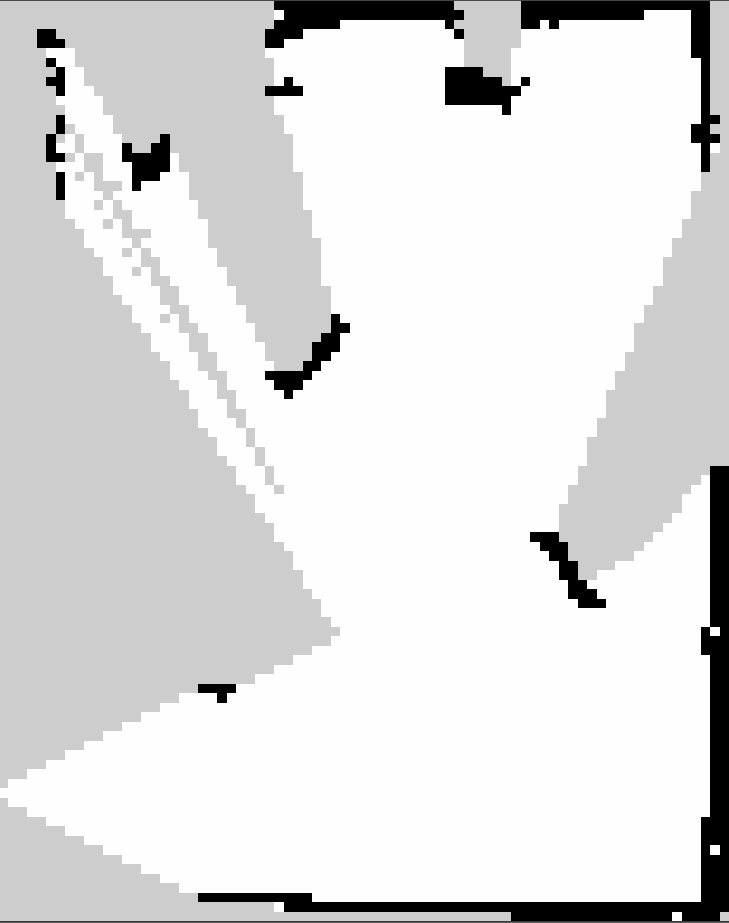
\includegraphics[width=0.8\linewidth]{figures/MAP.png}
	\caption{The map obtained in the video below}
	\label{fig:MAP}
\end{figure}
\href{https://youtu.be/gvVIIlhwI-I}{Here} is our attempt at testing slam\_toolbox alongside nav2. 
%=========================================================================================================================
%-------------- NAV2
%=========================================================================================================================
\subsection{Nav2}
Navigation in robotics refers to the ability of a robot to move from one location to another in an environment while avoiding obstacles and reaching its destination safely. The Nav2 project leverages ROS2 for building its navigation stack, which includes various components to enable mobile robot navigation.

\begin{enumerate}
    \item \textbf{Action Servers}: In the context of ROS2, action servers are used to manage long-running tasks that may take a significant amount of time to complete, such as navigation. They allow clients to request specific tasks, and the server provides feedback and results during the execution of the task. The Nav2 stack utilizes action servers extensively to handle navigation tasks, enabling efficient execution of complex actions like path planning and control.

    \item \textbf{Lifecycle Nodes and Bond}: ROS2 introduces the concept of lifecycle nodes, which are nodes that follow a state machine-based lifecycle. This helps in ensuring deterministic behavior during the startup and shutdown of ROS2 servers. The bond connection in Nav2 is used to ensure the active status of servers after they transition up. If a server crashes, the bond notifies the lifecycle manager, preventing critical failures.

    \item \textbf{Behavior Trees}: Behavior trees are a way of organizing complex robotics tasks in a hierarchical manner. In Nav2, the BehaviorTree CPP V3 library is used to construct behavior trees. These trees consist of various nodes representing specific behaviors or tasks. Behavior trees provide a formal structure for navigation logic and allow for the creation of complex systems while maintaining verifiability and validation.

    \item \textbf{Navigation Servers}: The Nav2 project employs several action servers to handle different aspects of navigation:
    \begin{itemize}
        \item \textbf{Planner Server}: Responsible for computing a valid path from the robot's current position to a goal location based on the global environmental representation.
        
        \item \textbf{Controller Server}: Handles local control efforts to follow the global plan or execute specific local tasks, like docking or avoiding obstacles.
        
        \item \textbf{Smoother Server}: Refines the path computed by the planner to improve its smoothness and overall quality.
        
        \item \textbf{Behavior Server}: Executes various recovery behaviors to deal with unknown or failure conditions, making the system more fault-tolerant.
    \end{itemize}

    \item \textbf{Waypoint Following}: Waypoint following is a fundamental feature of navigation systems. The Nav2 stack includes a waypoint following program with a plugin interface for executing specific tasks at multiple waypoints. It is useful for completing tasks like taking pictures, picking up objects, or waiting for user input at specified locations.

    \item \textbf{State Estimation}: State estimation involves determining the robot's pose (position and orientation) relative to a global reference frame. In Nav2, two main transformations are essential: \textcolor{Violet}{\texttt{map->odom}} and \textcolor{Violet}{\texttt{odom->base\_link}}. Global positioning systems (like GPS or SLAM) provide the \textcolor{Violet}{\texttt{map->odom}} transformation, while the odometry system (wheel encoders, IMUs, etc.) offers the \textcolor{Violet}{\texttt{odom->base\_link}} transformation.

    \item \textbf{Environmental Representation}: The environmental representation is how a robot perceives and models its surroundings. In Nav2, costmaps are used for this purpose. A costmap is a regular 2D grid that assigns costs to cells representing different types of areas (unknown, free, occupied, or inflated cost). Various costmap layers, implemented as pluginlib plugins, buffer information from sensors into the costmap to provide a comprehensive representation of the environment.

    \item \textbf{Costmap Filters}: Costmap filters in Nav2 are used to apply spatial-dependent behavioral changes based on annotations provided in filter masks. Filter masks contain data about specific areas in the environment where certain behaviors or restrictions should be applied. Costmap filters read this data and update the underlying costmap to alter the robot's behavior in those areas.
    
\end{enumerate}

Overall, Nav2 provides a powerful and flexible framework for mobile robot navigation within the ROS2 ecosystem, with support for various navigation-related concepts and components. \\


We specifically focus on optimizing the \textcolor{Plum}{\texttt{nav2\_velocity\_smoother}} for our task. In order to do that, we will need to understand the key parameters that influence the smoothing behavior. 

The \textcolor{Plum}{\texttt{nav2\_velocity\_smoother}} is a lifecycle-component node that is part of the Nav2 navigation stack. Its main purpose is to take in velocity commands from Nav2's controller server and apply smoothing to these commands before sending them to the robot's hardware controllers. It achieves this by taking input commands from the cmd\_vel topic and producing a smoothed output on the smoothed\_cmd\_vel topic.\\

Key features and design choices of the \textcolor{Plum}{\texttt{nav2\_velocity\_smoother}} node:
\begin{enumerate}
    \item \textbf{Lifecycle and Composition Management}: The node utilizes the ROS 2 lifecycle manager for state management, which ensures predictable behavior during startup, shutdown, and runtime. Additionally, it utilizes composition for process management, allowing it to work seamlessly with other components in the Nav2 stack.

    \item \textbf{Timer-based Smoothing}: Instead of simply computing a smoothed velocity command in the callback of each cmd\_vel input from Nav2, the node operates on a regular timer running at a configurable rate. This allows it to interpolate commands at a higher frequency than Nav2's local trajectory planners can provide. By running at a higher frequency, it provides a more regular stream of commands to the robot's hardware controllers and performs finer interpolation between the current velocity and the desired velocity. This results in smoother acceleration and motion profiles, leading to better overall performance.

    \item \textbf{Open and Closed Loop Operation Modes}: The node supports two primary operation modes:
    \begin{itemize}
        \item \textbf{\textit{Open-loop}}: In this mode, the node assumes that the robot was able to achieve the velocity sent to it in the last command, which has been smoothed. This assumption is valid when acceleration limits are set properly. It is useful when robot odometry is not particularly accurate or has significant latency relative to the smoothing frequency. In open-loop mode, there is no delay in the feedback loop.
        \item \textbf{\textit{Closed-loop}}: In this mode, the node reads from the odometry topic and applies a smoother over it to obtain the robot's current speed. This current speed is then used to determine the robot's achievable velocity targets, taking into account velocity, acceleration, and deadband constraints using live data.
    \end{itemize}    
\end{enumerate}

The \textcolor{Plum}{\texttt{nav2\_velocity\_smoother}} node plays a crucial role in enhancing the performance of robot motion control. By smoothing the velocity commands, it reduces jerky movements and wear-and-tear on robot motors and hardware controllers. The ability to operate in different modes allows flexibility in adapting to various robot setups and odometry accuracy levels. Overall, this node is a valuable component in the Nav2 navigation stack, contributing to the smooth and efficient navigation of mobile robots.

The \textcolor{Plum}{\texttt{nav2\_velocity\_smoother}} is responsible for smoothing velocities to reduce wear-and-tear on robot motors and hardware controllers by mitigating jerky movements resulting from some local trajectory planners' control efforts. The main \textcolor{Plum}{\texttt{nav2\_velocity\_smoother}} parameters that we adjust on are:
\begin{itemize}
    \item \texttt{\textcolor{OliveGreen}{'smoothing\_frequency'}: \textcolor{NavyBlue}{0.1}}\\
    \textit{This parameter controls how quickly the velocity is adjusted to smooth out accelerations and jerky movements. A lower smoothing frequency will result in slower adjustments, while a higher smoothing frequency will make the smoothing more responsive.}
    
    \item \texttt{\textcolor{OliveGreen}{'scale\_velocities'}: \textcolor{NavyBlue}{True}}\\
    \textit{When set to true, this parameter adjusts other components of velocity proportionally to a component’s required changes due to acceleration limits. It tries to make all components of velocity follow the same direction, but still enforces acceleration limits to guarantee compliance, even if it means deviating off the commanded trajectory slightly. This can help in maintaining a smoother and more coordinated motion of the robot.}
    
    \item \texttt{\textcolor{OliveGreen}{'feedback'}: \textcolor{OliveGreen}{'OPEN\_LOOP'}}
    
    \item \texttt{\textcolor{OliveGreen}{'max\_velocity'}: [\textcolor{OliveGreen}{1.4, 0.0, 0.2}]}
    
    \item \texttt{\textcolor{OliveGreen}{'min\_velocity'}: [\textcolor{OliveGreen}{-1.4, 0.0, -0.2}]}\\
    \textit{In some cases, you may want to set a minimum velocity to ensure the robot continues moving even in low-speed situations. This can be useful for preventing the robot from coming to a complete stop during trajectory planning.}
    
    \item \texttt{\textcolor{OliveGreen}{'max\_accel'}: [\textcolor{OliveGreen}{1.125, 0.0, 1.125}]}\\
    \textit{This parameter limits the rate at which the linear and angular velocities can change. By constraining the accelerations, you can prevent sudden and abrupt changes in velocity.}
    
    \item \texttt{\textcolor{OliveGreen}{'max\_decel'}: [\textcolor{OliveGreen}{-1.125, 0.0, -1.125}]}
    
    \item \texttt{\textcolor{OliveGreen}{'deadband\_velocity'}: [\textcolor{OliveGreen}{0.0, 0.0, 0.0}]}\\
    \textit{The deadband is a small range around zero velocity where no adjustments are made. This parameter sets the minimum velocities (m/s) to send to the robot hardware controllers to prevent small commands from damaging hardware controllers if that speed cannot be achieved due to stall torque. It helps avoid applying very small velocities that might lead to wear-and-tear on the robot hardware.}
    
\end{itemize}
%=========================================================================================================================
%-------------- vSLAM
%=========================================================================================================================
\subsection{vSLAM}
The development of 2D laser scanners was a game-changer for robotics, but their high cost has become a bottleneck for widespread adoption. To enable the next wave of robot applications, more affordable RGB-D sensors and cameras are crucial, especially in challenging environments where 2D techniques are not suitable. These advancements will allow for broader robot deployment and address new problems in various industries. 

Some vSLAM approaches that we considered include:
\begin{itemize}
    \item \textbf{ORB-SLAM3}: ORB-SLAM3 is a versatile visual SLAM method designed to work with various sensors, including monocular, stereo, and RGB-D cameras. ORB-SLAM has often adapted to enhance odometry systems for service robots. The latest version, ORB-SLAM3, introduces significant improvements, such as visual-inertial SLAM, allowing sensor fusion of visual and inertial sensors for more robust tracking in challenging environments with fewer point features. It also supports multi-map continuation and fisheye camera compatibility, expanding its applicability to different camera types.

    \item \textbf{RTABMap}: RTABMap is one of the oldest mixed-modality SLAM approaches. It stands out for its flexibility in accepting various input sensors, including stereo, RGB-D, fish-eye cameras, odometry, and 2D/3D lidar data. Unlike traditional feature-based SLAM methods, RTABMap creates dense 3D and 2D representations of the environment, making it unique and highly compatible as a semi-visual SLAM replacement. This characteristic allows for seamless integration into existing systems without additional post-processing, offering a compelling advantage.

    \item \textbf{OpenVSLAM}: OpenVSLAM is a well-structured implementation of ORB feature-based Visual graph SLAM. It offers optimized feature extractors and stereo matchers, alongside a unique frame tracking module for fast and accurate localization, competing with state-of-the-art solutions. The versatility of OpenVSLAM allows it to work with various camera models, including equirectangular and fisheye, making it suitable for a wide range of applications.
\end{itemize}

In the end, we opted for RTABMap for our ground robot experiments in a low-featured indoor facility equipped with an RGB-D camera. 

\subsubsection*{RTAB-Map}
RTAB-Map (Real-Time Appearance-Based Mapping) is a Graph SLAM approach that utilizes RGB-D data for real-time mapping. It employs a global Bayesian loop closure detector to efficiently detect and close loops in the mapping process. RTAB-Map can function independently with a handheld Kinect or stereo camera to perform 6DoF (degrees of freedom) RGB-D mapping. Alternatively, it can be used on a robot equipped with a laser rangefinder for 3DoF mapping with a 2D LiDAR or 6DoF mapping with a 3D LiDAR.\\

In the context of ROS, RTAB-Map is available as a package that serves as a wrapper for the RTAB-Map SLAM approach. This ROS package enables seamless integration and use of RTAB-Map with ROS-based systems. Various additional packages are available that can work in conjunction with RTAB-Map to generate 3D point clouds of the environment or create 2D occupancy grid maps, which are useful for navigation tasks.

In our specific case, where we have an RGB-D camera, odometry information from wheel encoders, and fake laser scans generated from depth images, we fine-tuned RTABMap's parameters to achieve optimal performance and accuracy. Here's how we adjusted the parameters.

\begin{figure}[H]
	\centering
	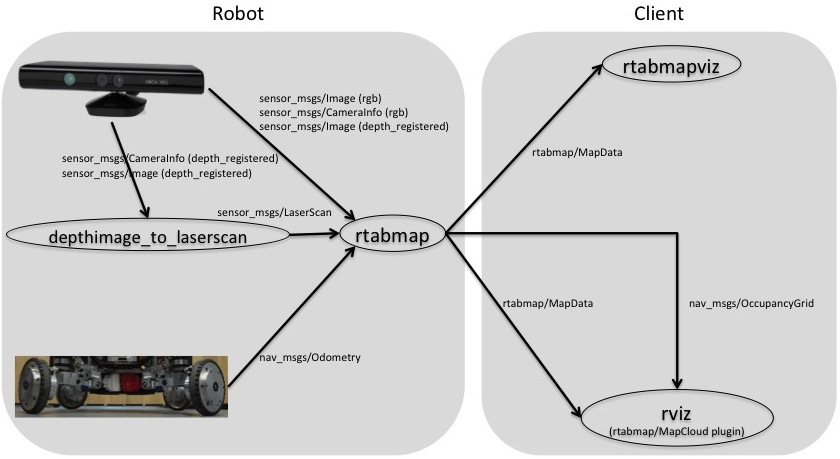
\includegraphics[width=0.8\linewidth]{figures/rtabmap-config.png}
	\caption{\href{http://wiki.ros.org/rtabmap_ros/Tutorials/SetupOnYourRobot}{Kinect + Odometry + Fake 2D laser from Kinect}}
	\label{fig:rtabmap-config}
\end{figure}


For RTABMap's ROS wrapper parameters:
\begin{itemize}
    \item \texttt{\textcolor{LimeGreen}{'subscribe\_depth'}: \textcolor{NavyBlue}{True}}\\
    \textit{Subscribe to depth image}
    \item \texttt{\textcolor{LimeGreen}{'subscribe\_scan'}: \textcolor{NavyBlue}{True}}\\
    \textit{Subscribe to laser scan}
    \item \texttt{\textcolor{LimeGreen}{'subscribe\_rgbd'}: \textcolor{NavyBlue}{False}}\\
    \textit{Subsribe to rgbd\_image topic.}
    \item \texttt{\textcolor{LimeGreen}{'qos\_image'}: LaunchConfiguration(\textcolor{LimeGreen}{'qos'})}
    \item \texttt{\textcolor{LimeGreen}{'qos\_scan'}: LaunchConfiguration(\textcolor{LimeGreen}{'qos'})}
    \item \texttt{\textcolor{LimeGreen}{'use\_action\_for\_goal'}: \textcolor{NavyBlue}{True}}\\
    \textit{Planning Use actionlib to send the metric goals to move\_base. The advantage over just connecting goal\_out to move\_base\_simple/goal is that rtabmap can have a feedback if the goal is reached or if move\_base has failed.}
    \item \texttt{\textcolor{LimeGreen}{'approx\_sync'}: \textcolor{NavyBlue}{True}}\\
    \textit{Use approximate time synchronization of input messages. If false, note that the odometry input must have also exactly the same timestamps than the input images.}
    \item \texttt{\textcolor{LimeGreen}{'tf\_delay'}: \textcolor{NavyBlue}{4.0}}\\
    \textit{Rate at which the TF from /map to /odom is published}
\end{itemize}

For most of UGV, the vehicle only runs on a flat ground, in this way, you can force the visual odometry to track the vehicle in only 3DOF (x,y,theta) and increase the robustness of the map. For rtabmap, we can also constraint to 3 DoF loop closure detection and graph optimization:

For RTABMap's parameters:
\begin{itemize}
    \item \texttt{\textcolor{LimeGreen}{'Optimizer/Strategy'}: \textcolor{LimeGreen}{'1'}}\\
    \textit{Graph optimization strategy: 0=TORO, 1=g2o, 2=GTSAM and 3=Ceres.}
    \item \texttt{\textcolor{LimeGreen}{'RGBD/ProximityBySpace'}: \textcolor{LimeGreen}{'false'}}\\
    \textit{Detection over locations (in Working Memory) near in space.}
    \item \texttt{\textcolor{LimeGreen}{'Reg/Force3DoF'}: \textcolor{LimeGreen}{'true'}}
    \item \texttt{\textcolor{LimeGreen}{'Vis/MinInliers'}: \textcolor{LimeGreen}{'12'}}\\
    \textit{Minimum feature correspondences to compute/accept the transformation.}
    \item \texttt{\textcolor{LimeGreen}{'RGBD/AngularUpdate'}: \textcolor{LimeGreen}{'0.01'}}\\
    \textit{Minimum angular displacement (rad) to update the map. Rehearsal is done prior to this, so weights are still updated.}
    \item \texttt{\textcolor{LimeGreen}{'RGBD/LinearUpdate'}: \textcolor{LimeGreen}{'0.01'}}\\
    \textit{Minimum linear displacement (m) to update the map. Rehearsal is done prior to this, so weights are still updated.}
    \item \texttt{\textcolor{LimeGreen}{'RGBD/OptimizeFromGraphEnd'}: \textcolor{LimeGreen}{'false'}}\\
    \textit{Optimize graph from the newest node. If false, the graph is optimized from the oldest node of the current graph (this adds an overhead computation to detect to oldest node of the current graph, but it can be useful to preserve the map referential from the oldest node). Warning when set to false: when some nodes are transferred, the first referential of the local map may change, resulting in momentary changes in robot/map position (which are annoying in teleoperation).}
\end{itemize}

By fine-tuning these parameters, we were able to tailor RTABMap to our specific setup. This process allowed us to achieve reliable and accurate SLAM results in our low-featured indoor facility.